
\item A parallel plate capacitor has a dielectric slab of dielectric constant \(K\) between its plates that covers \(1/3\) of the area of its plates, as shown in the figure. The total capacitance of the capacitor is \(C\) while that of the portion with dielectric in between is \(C_1\). When the capacitor is charged, the plate area covered by the dielectric gets charge \(Q_1\) and the rest of the area gets charge \(Q_2\). The electric field in the dielectric is \(E_1\) and that in the other portion is \(E_2\). Choose the correct option/options, ignoring edge effects.
    \begin{center}
        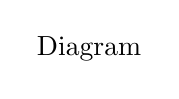
\begin{tikzpicture}
            % Diagram can be implemented by an artist or using TikZ commands depending on the requirement.
            \node at (0, 0) {Diagram};
        \end{tikzpicture}
    \end{center}
    \begin{tasks}(2)
        \task \(\frac{E_1}{E_2} = 1\)
        \task \(\frac{E_1}{E_2} = \frac{1}{K}\)
        \task \(\frac{Q_1}{Q_2} = \frac{3}{K}\)
        \task \(\frac{C}{C_1} = \frac{2+K}{K}\)
    \end{tasks}
